\chapter{Numerical Implementation}\label{chap:Numerical}

Since this modern era of fission theory takes advantage of high-performance computers, it is worth taking some time to discuss some of the issues which came up during the course of this research, and how modern computing tools were used to solve the problem.

\section{Calculating the PES}
By far, the most time-intensive part of a microscopic fission calculation is the calculation of the PES. For this we use a pair of DFT solvers, HFODD~\cite{Schunck2017} and HFBTHO~\cite{Perez2017}. These programs solve the HFB equations in a basis of deformed harmonic oscillators. The solver HFBTHO is limited to shapes with axial symmetry, while HFODD allows for the breaking of any symmetry needed. Broken symmetries mean that each matrix element must be computed independently, while good symmetries reduce the number of calculations which must be performed. However, since the major bottleneck of each of these programs involves constructing matrices representing Skyrme densities and currents and then diagonalizing the matrix representing the HFB Hamiltonian, this flexibility drastically increases the time-to-solution.

On the positive side, the problem of calculating a PES is embarrassingly-parallel. So while an individual point in the PES may be difficult to compute, many points can be computed simultaneously. This does have its limitations; highly-deformed configurations may be very unstable because of reasons. One fix may sometimes be to use a nearby point which converged successfully as a seed function

The procedure is performed iteratively: First, an ansatz is given for the density (either by the user or by some simple means, such as a quick Woods-Saxon calculation). Then the energy density matrix is constructed, after which it is diagonalized and a new density matrix is calculated. The procedure then repeats for a fixed number of iterations, or until a predetermined convergence criterion is satisfied In HFODD, for instance, the default convergence criterion is for the difference between the HFB energy and the total energy summed over all single-particle states to be less than some user-defined value.

%Certain parts of the procedure can be parallelized using shared-memory parallelism, such as QMULCM, which does what again? It readjusts the Lagrange parameters of the constraints based on the perturbative approximation fot he QRPA matrix.

\subsection{PES Tools}
Apart from the issue of walltime, generating a PES creates a lot of output files, which quickly becomes unwieldy. To help manage all this data, a Python module called PES Tools was created for manipulating, extracting, interpolating, and plotting PES data~\cite{PES_tools}. Aside from solver-dependent parser scripts, which collect data from the output of a DFT run and store it in the XML file format, PES Tools is not dependent on a particular DFT solver.

In particular, a submodule was created to interface between PES Tools and Fission Tools~\cite{fission_tools}, a set of codes which have relevance to fission calculations. Many of these codes are described in the following sections.

\section{Calculating the collective inertia}\label{sect:M_numerical}
The partial derivatives from equation \eqref{eq:mATDHFB-np} are computed using the Lagrange three-point formula:

\begin{equation}\label{eq:finite-diffs}
\left(\frac{\partial \mathcal{R}}{\partial q}\right)_{q=q_0} \approx 
    \frac{-\delta q'}{\delta q \left(\delta q + \delta q'\right)}\mathcal{R}(q_0-\delta q) + 
    \frac{\delta q - \delta q'}{\delta q \delta q'}\mathcal{R}(q_0) + 
    \frac{\delta q}{\delta q' \left(\delta q + \delta q'\right)}\mathcal{R}(q_0+\delta q')
\end{equation}

The accuracy and precision of the collective inertia $\mathcal{M}$ are therefore functions of the spacings $\delta q$ and $\delta q'$, and of $\mathcal{R}$. An accurate value of the collective inertia is especially important for computing half-lives, where there is an exponential dependence on $\mathcal{M}$.

\begin{figure}
	\centering
	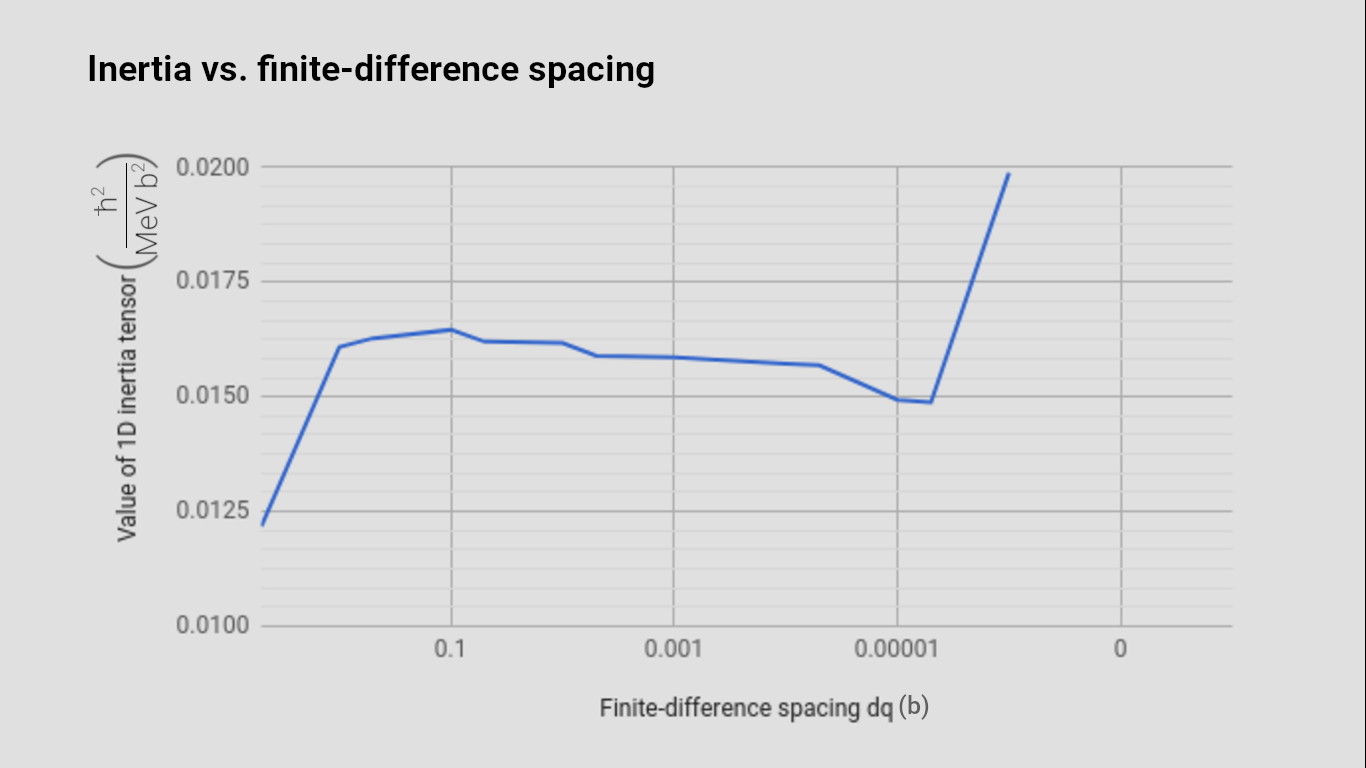
\includegraphics[width=0.7\linewidth]{TeX_files/Num-dq_spacing}
	\caption[Collective inertia as a function of finite-difference spacing]{$\mathcal{M}_{22}$ calculated for an arbitrary configuration of $^{240}$Pu as a function of finite-difference spacing.}
	\label{fig:num-dqspacing}
\end{figure}

Figure~\ref{fig:num-dqspacing} shows the effect of different values of $\delta q = \delta q'$ on the collective inertia for an arbitrary configuration of $^{240}$Pu.

\begin{figure}
	\centering
	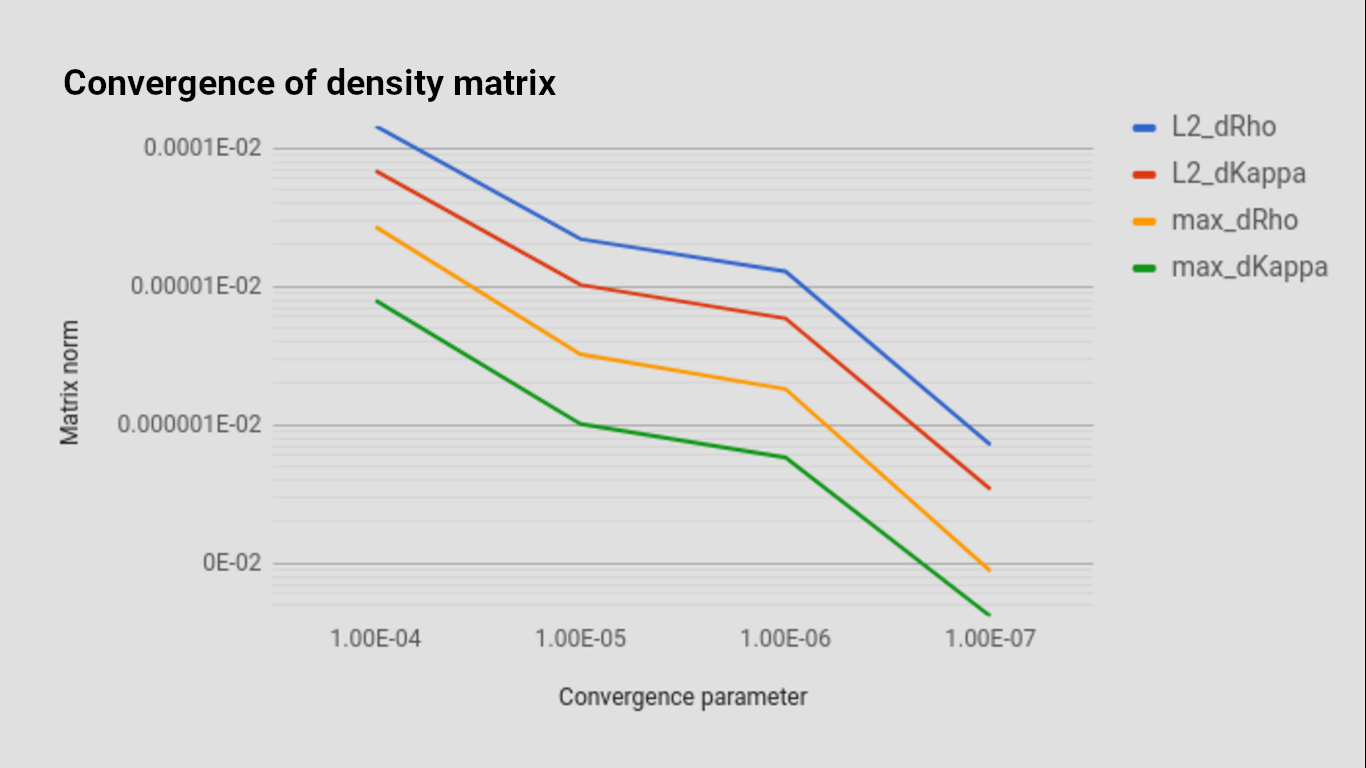
\includegraphics[width=0.7\linewidth]{TeX_files/Num-rho_conv}
	\caption[Norm of the difference matrix between subsequent iterations of the density]{Norm of the difference matrix between subsequent iterations of the density.}
	\label{fig:num-rhoconv}
\end{figure}

Figure~\ref{fig:num-dqspacing} shows the norm of the matrix which corresponds to the difference between the density matrix at the last iteration and the second-to-last iteration. Predictably, the norm decreases as the convergence parameter becomes tighter. This gives a sense of the uncertainty associated with the density, which in turn should be propagated through equations \eqref{eq:finite-diffs} and \eqref{eq:mATDHFB-np}.

There are additional complications which arise in the finite-temperature formalism. These are discussed in Appendix~\ref{append:TD-ATDHFB}.

\section{Minimum action path}
For the tunneling described in Section~\ref{sect:wkb}, the dynamic programming method~\cite{Baran1981} was used to minimize the action. The dynamic programming scheme proceeds inductively: Once the minimum action is known for all grid points up to a certain value of $Q_{20}$, say $q_{20}^n$, then the minimum action at each grid point in the layer with $Q_{20}=q_{20}^{n+1}$ is obtained by computing the action between each grid point in layer $n$ and each grid point in layer $n+1$, and then finding the path which minimizes the total action at each grid point in layer $n+1$:

\begin{equation}
\left.S_{min}(\vec{Q})\right|_{Q_{20}=q_{20}^{n+1}} = \mathrm{argmin}_{\vec{Q'}}\left.\left(S_{min}(\vec{Q'}) + \Delta S_{min}(\vec{Q},\vec{Q'})\right)\right|_{Q'_{20}=q_{20}^{n}, Q_{20}=q_{20}^{n+1}}.
\end{equation}

The inductive step which connects layers $n$ and $n+1$ involves several small, independent calculations which lend themselves well to shared-memory parallelism. This was implemented in the code using OpenMP, resulting in a walltime reduction from order $\mathcal{O}(n^D)$ to $\mathcal{O}(n^D/m)$, where $m$ is the number of processors (with the usual caveats that parallelization requires some additional overhead time, and that the actual speedup might be somewhat less when the number of processors $m$ reaches the same order as the number of points per layer $n^{D-1}$). In a 2D calculation, where the runtime is on the order of seconds, the difference is inconsequential. However, this speedup was essential for the analysis of a 4D PES, as described in Chapter~\ref{chap:294Og}.


\section{Langevin}
Once the action and relative probability are known for a set of points along the outer turning line, Langevin trajectories are computed originating from each outer turning point. These are straightforwardly evaluated at discrete time steps over a discretized PES mesh.

Because of the random force term in equation \eqref{eq:langevin}, a large number of trajectories per outer turning point must be computed to reduce statistical uncertainty. Fortunately, each trajectory is completely independent of every other trajectory, lending the code readily to shared-memory parallelism. However, for the Fission Tools Langevin code, distributed-memory parallelism was chosen over shared-memory parallelism in order to simplify access to shared resources, such as variables and output files.